\subsection{Afbeeldingen}
\pvelist{ \pve{2.15} }

Afbeeldingen worden automatisch geschaald in verhouding naar aanleiding van het design. De originele afbeelding wordt bewaard op de server: Een voorbeeld:

Originele afbeelding: http://accept.prorail.nl.kpnis.nl/sites/default/files/nachtelijk\_onderhoud\_aan\_het\_spoor\_300dpi\_451x300mm\_c.jpg
Geschaald: http://accept.prorail.nl.kpnis.nl/sites/default/files/styles/960x437/public/nachtelijk\_onderhoud\_aan\_het\_spoor\_300dpi\_451x300mm\_c.jpg

Als er een afbeelding wordt toegevoegd in de WYSIWYG editor heeft de gebruiker de keuze om drie formaten te kiezen:

\begin{enumerate}
\item Standaard, De afbeelding wordt net zo groot als het content vlak
\item Teaser, De afbeelding wordt net zo groot als een afbeelding in het overzicht
\item Origineel, De afbeelding wordt net zo groot als het is geupload
\end{enumerate}

\begin{figure}[p]
\centering
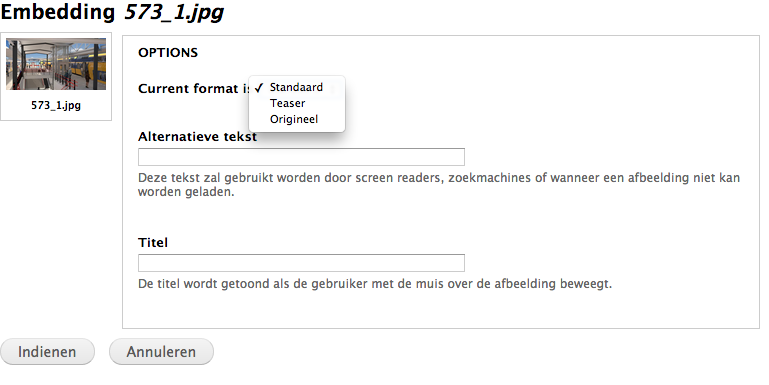
\includegraphics[width=\textwidth]{img/wysiwyg_image.png}
\caption{De drie aanwezige formaten om een afbeelding toe te voegen aan de tekst}
\label{fig:felix_image}
\end{figure}

Bij het toevoegen van afbeeldingen bij bijvoorbeeld een nieuwsartikel, heeft de redacteur de mogelijkheid om een fotoalbum te maken. Als de redacteur meer dan 1 afbeelding aan het nieuwsbericht toevoegt verschijnt er automatisch bij dat nieuwsbericht een fotoalbum.

Afbeeldingen via Flickr kunnen toegevoegd worden via de embed code van Flickr.

Om Flickr sets toe te voegen op de website kan door middel van Felix. Kies hiervoor voor Flickr set en vul het gebruikersnummer en de setnummer in.